
\chapter{Plots}
\label{ch:plots}
\newgeometry{inner=2.5cm,outer=2.5cm,bottom=2.5cm,top=0.5cm}


\begin{figure}
\makebox[\textwidth][c]{
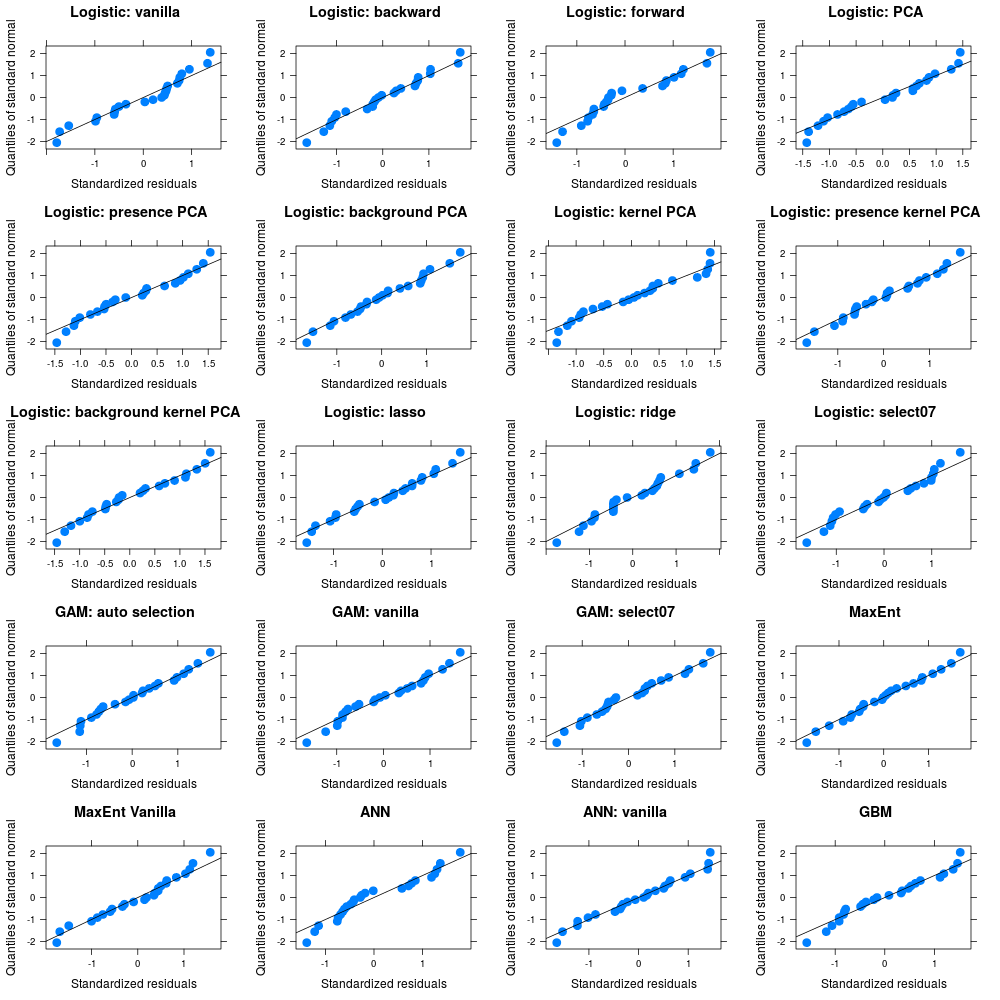
\includegraphics[scale=.6]{Plots/ResidualPlotsGLS.png}
}
\caption{\label{fig:ResidualGLSAll}QQ-plot of the residuals of the GLS model for the models fitted on all the variables.}
\end{figure}


\begin{figure}
\makebox[\textwidth][c]{
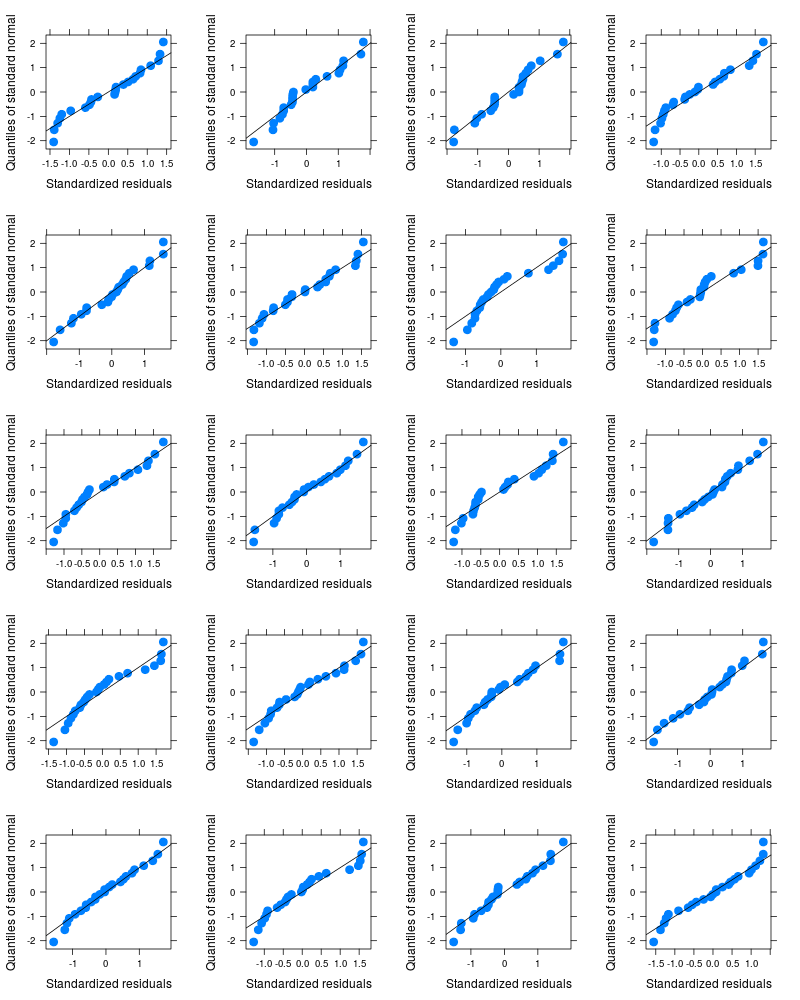
\includegraphics[scale=.6]{Plots/ResidualPlotGLSBio.png}
}
\caption{\label{fig:ResidualGLSBio}QQ-plot of the residuals of the GLS model for the models fitted with only the bioclimatic variables.}
\end{figure}

\begin{figure}
\makebox[\textwidth][c]{
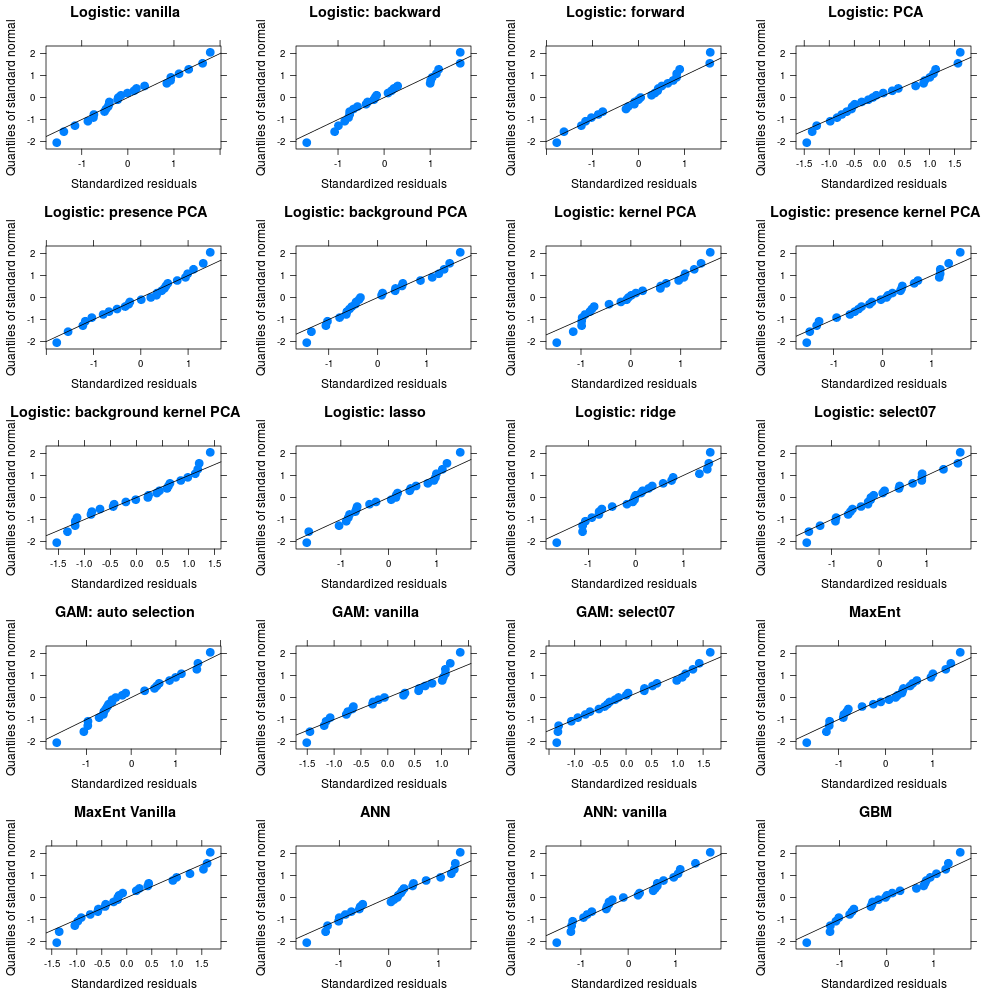
\includegraphics[scale=.6]{Plots/ResidualPlotGLSDiff.png}
}
\caption{\label{fig:ResidualGLSDiff}QQ-plot of the residuals of the GLS model for difference between the models fitted on the all variables versus only the bioclimatic variables.}
\end{figure}

\begin{figure}
\makebox[\textwidth][c]{
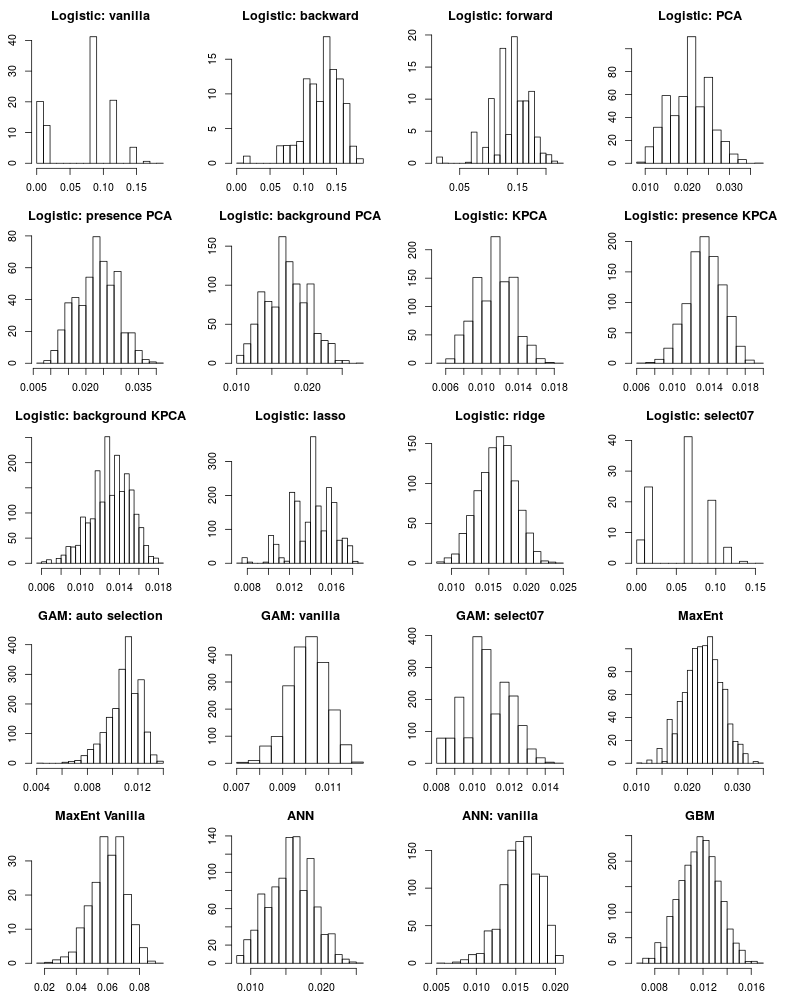
\includegraphics[scale=.7]{Plots/BootstrapAll.png}
}
\caption{\label{fig:BootstapAll}Histogram of the bootstrap sample of $\hat{\tau}$ when all variables are used.}
\end{figure}
\begin{figure}
\makebox[\textwidth][c]{
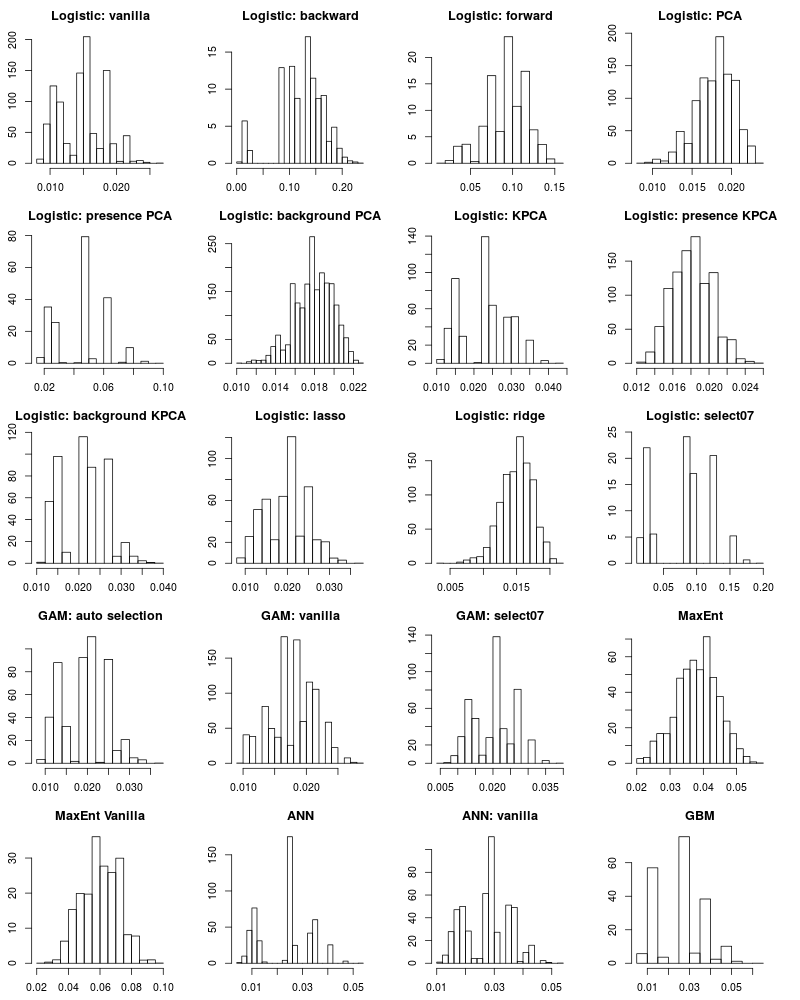
\includegraphics[scale=.7]{Plots/BootstrapBio.png}
}
\caption{\label{fig:BootstapBio}Histogram of the bootstrap sample of $\hat{\tau}$ when only the bioclimatic variables are used.}
\end{figure}

\begin{figure}
\makebox[\textwidth][c]{
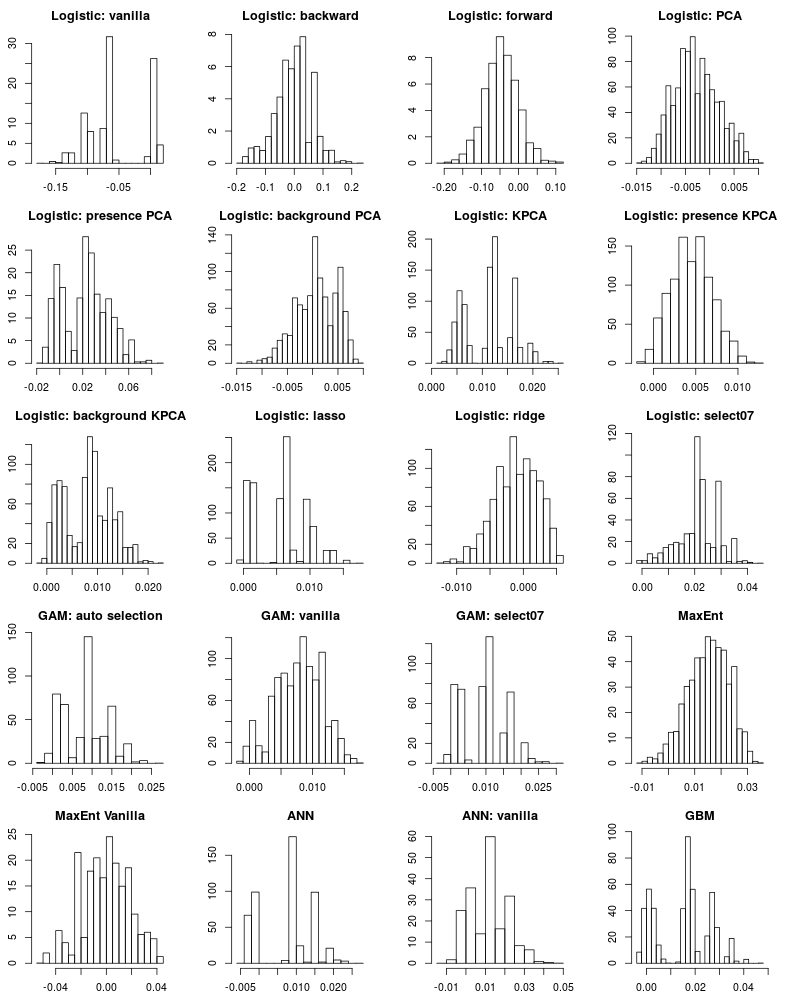
\includegraphics[scale=.7]{Plots/BootstrapDiff.png}
}
\caption{\label{fig:BootstapDiff}Histogram of the bootstrap sample of $\hat{\tau}_{bio} - \hat{\tau}_{all}$.}
\end{figure}

\restoregeometry